\section{Processes to synchronize model and code}
\label{sec:processes}

%Model-driven engineering has been established as a potential approach to gain software quality and productivity \cite{Mussbacher2014}. 
This section shows our use cases and scenarios in the collaboration of model-driven developers and traditional developers. The scenario 1 and 2 show how simple forward and reverse engineering combined to a create a RTE supported by most round-trip engineering tools such as 

\subsection{Scenario 1: modifications only made to code}
\label{scenario1}

The scenario 1 occurs when a group of people consisting of software architects, model-driven developers and traditional developers (programmers) have a need to create a software based on a legacy system or some legacy code that programmers are working with and want to directly contribute to the system description in order to gain quality. In the first step, it is of course not easy to communicate the stakeholders in the group. To have better understanding of the legacy system, a traditional reverse engineering is enough. 

In Fig. \ref{fig:scenario1}, the step (1) is to reverse the legacy code of the legacy system to a model. This scenario has a possible variant in case of not having an existing legacy system and the model is created from scratch. Based on the diagrams rendered the step (1), the stakeholders can discuss the system overall and ask programmers what to do in the legacy code. Nevertheless, this traditional development method does not profit the advantages of Model-driven engineering that allows to generate code and provides better organization. Therefore, we have a step (2) to modifying or re-factoring the created model to have a better architecture of the system and generating code from the model. The programmers then work with this generated code rather than the legacy code in the step (3). The architects and model-driven developers then reverse engineer the evolved code back to the model by an overwriting and analyze the system by using the new model in the step (4). The steps (2) and (4) are supported by many research prototypes and commercial tools \cite{UModel, visual, Rhapsody, Magicdraw, EA} but the model created in the step (4) is usually a surprise to architects since its diagrams are rendered differently from the original model. To handle this problem, it is necessary to preserve diagrams' properties of the original model by an incremental reverse engineering in the step (4) which is limitedly supported by most of the tools. 

\begin{figure}
\centering
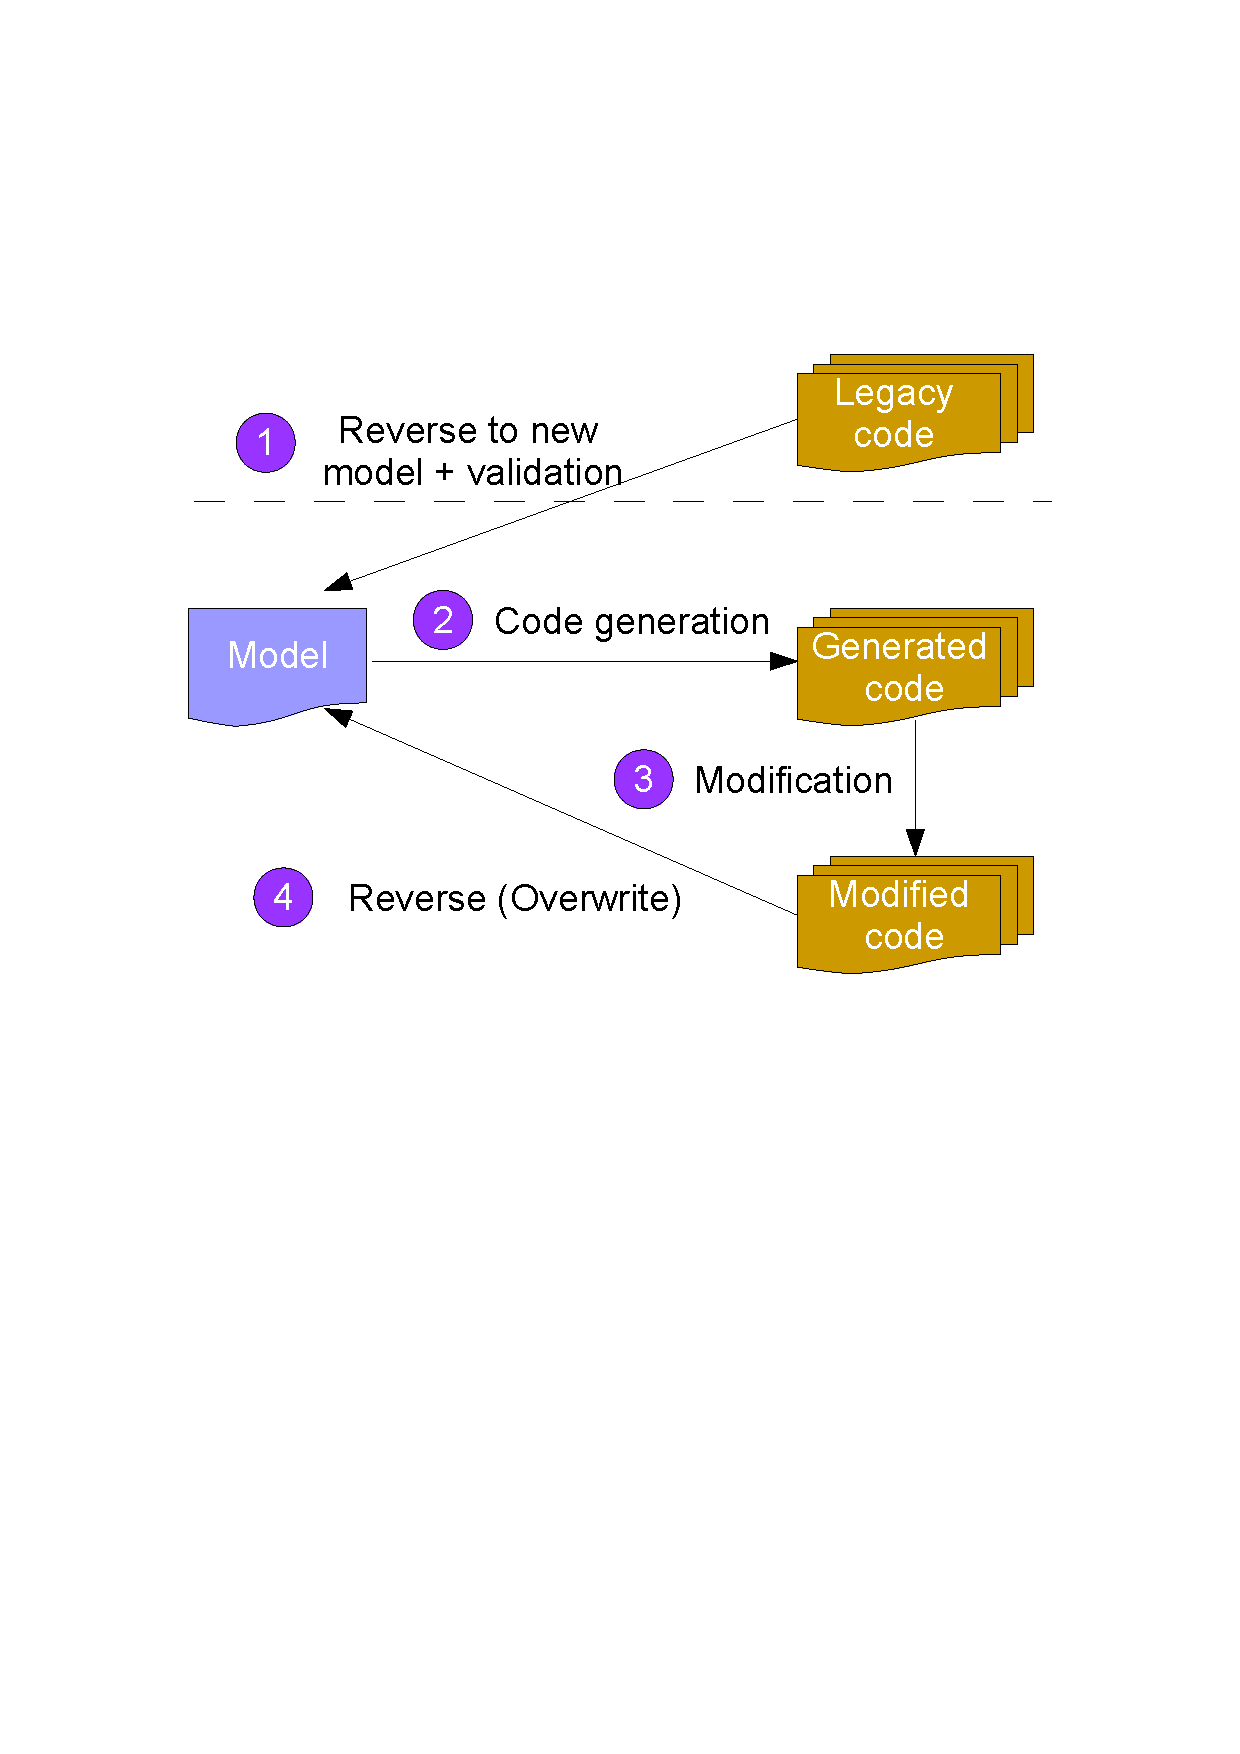
\includegraphics[height = 0.20\textheight, trim = 90 370 60 170, clip]{figures/scenario1}
\caption{\label{fig:scenario1}Round-trip engineering in case only code is modified} 
\end{figure}

\subsection{Scenario 2: modifications only made to model}
\label{scenario2}
The scenario 2 is similar to the scenario 1 in the first two steps (see Fig. \ref{fig:scenario2}. The difference is that instead of changing the generated code, MDE developers make modifications on the model. This scenario is close to re-engineering \cite{Chikofsky1990} of a software system by using MDE paradigm. In order to make the modified model and code consistent again, a code generation is needed in the step (4). The batch generation is supported by many tools as mentioned in the sub-section \ref{scenario1}, incremental code generation is still missing in these tools.  

\begin{figure}
\centering
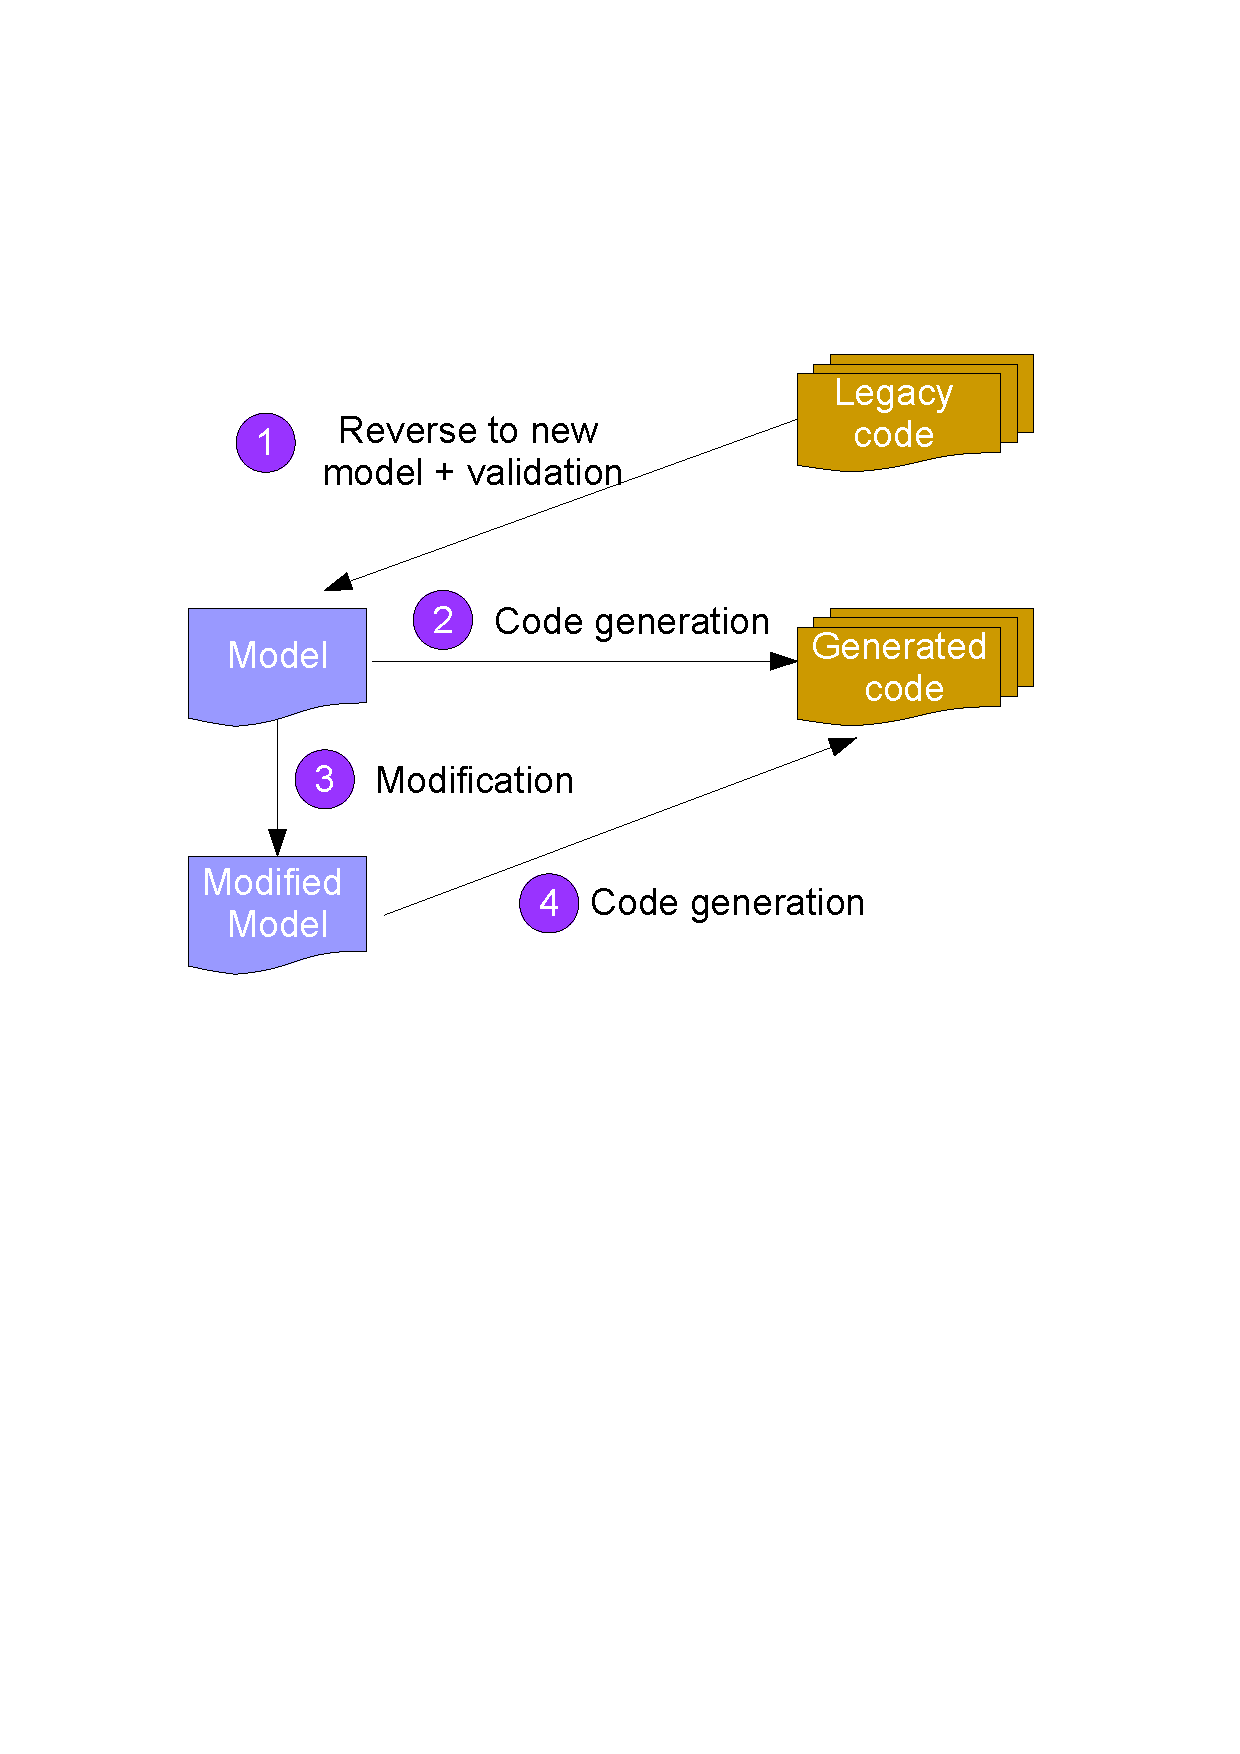
\includegraphics[height = 0.20\textheight, trim = 90 370 60 170, clip]{figures/scenario2}
\caption{\label{fig:scenario2}Round-trip engineering in case only model is modified} 
\end{figure}


\subsection{Scenario 3: concurrent modifications}
\label{scenario3}
The beauty of MDE is that it allows not only programmers but all different stakeholders concurrently contribute to the system description that is in turn translated to code. This ability gains software quality and productivity. This is where the scenario 3 stems from. Let's imagine that after creating software model by reverse engineering in the step (1) in Fig. \ref{fig:scenario3}, software architects may change the system architecture by re-factoring and in the meantime, traditional programmers might delete or add more methods/attributes or simple change methods' behavior. The modified model and code are then out of synchronization. The gap between the model and code makes the two profiles inconsistent: one artifact is non-sense to the other. This inconsistency in turn reduces the software quality. Therefore, a real synchronization is needed in the step (4). 

\begin{figure}
\centering
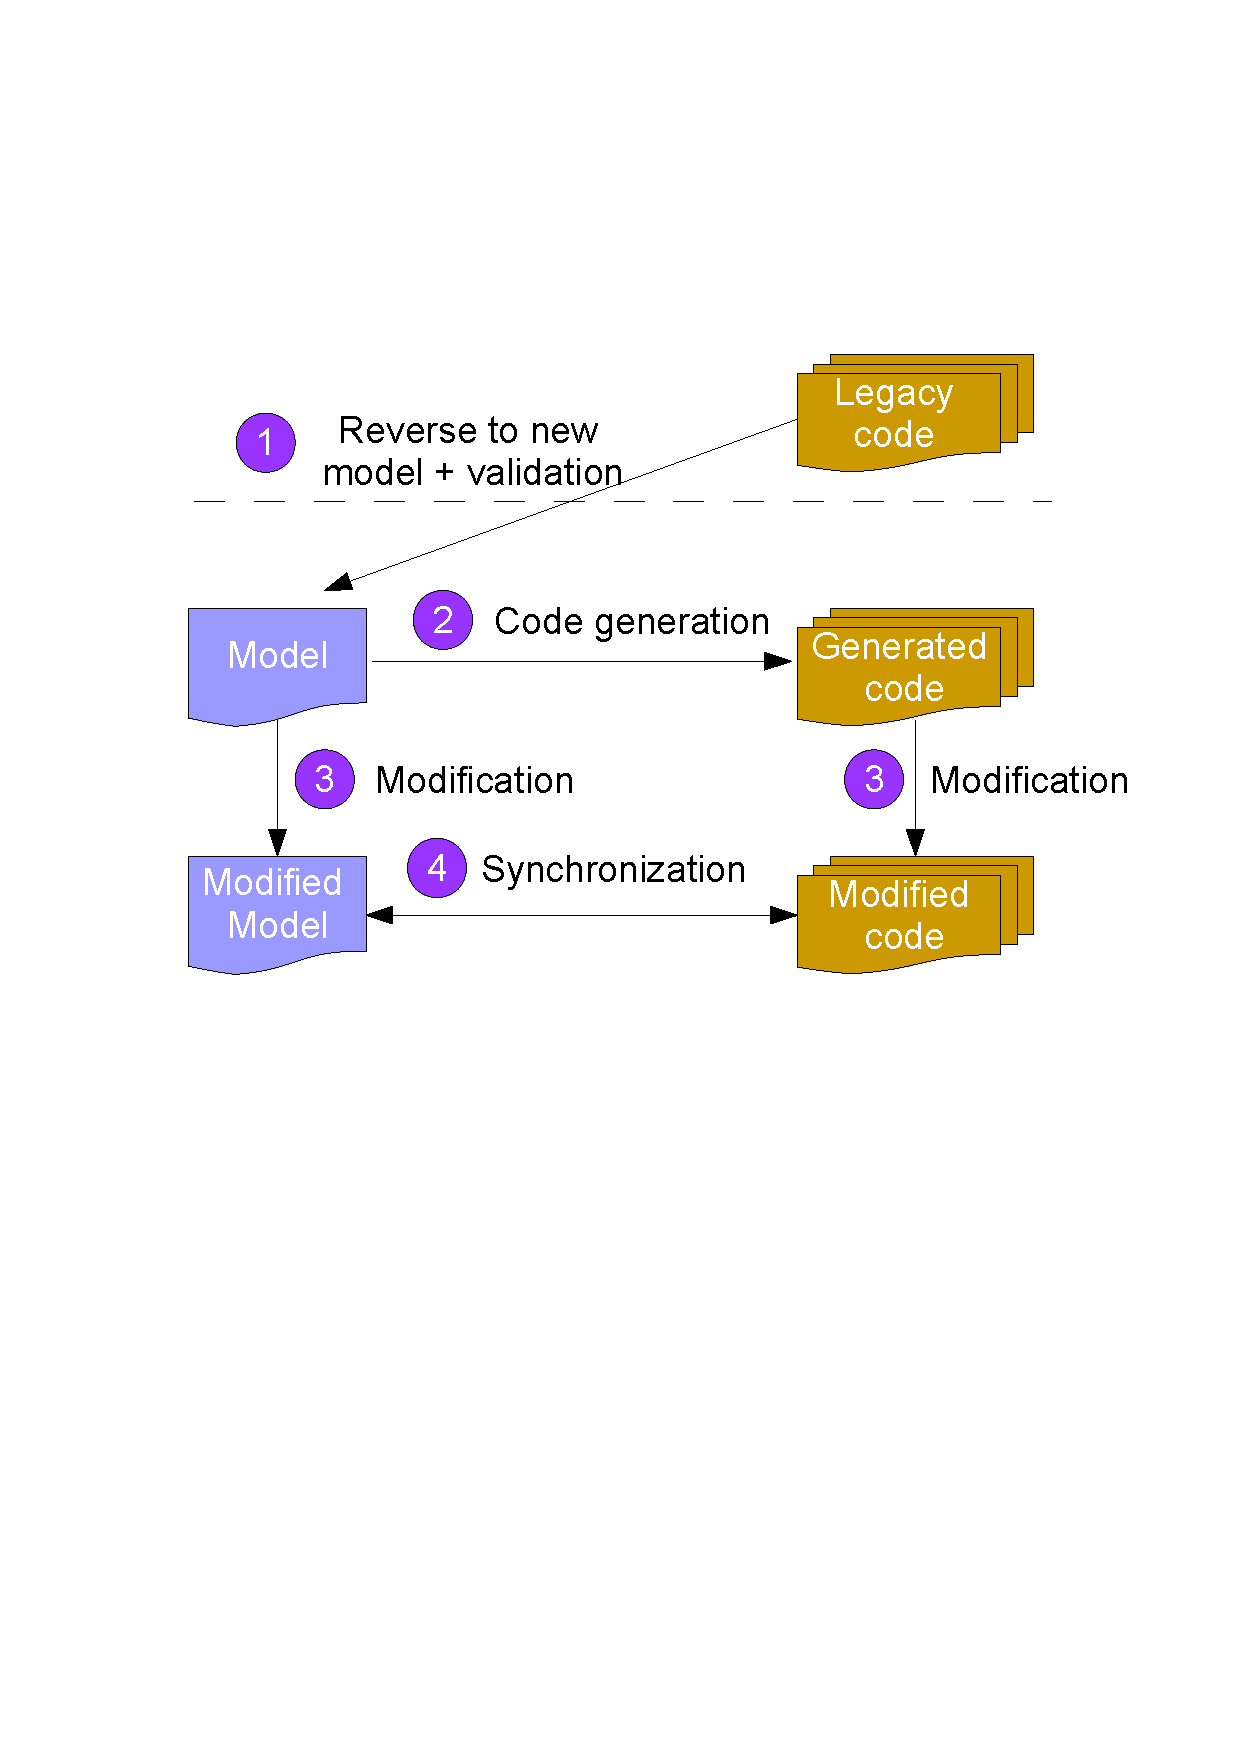
\includegraphics[height = 0.20\textheight, trim = 90 370 60 170, clip]{figures/scenario3}
\caption{\label{fig:scenario3}Model and code are concurrently modified} 
\end{figure}